\section{Auswertung}
\label{sec:Auswertung}
%Quellen programme.bib?

\subsection{Überprüfung der Stabilitätsbedingung}

Im ersten Teil des Versuchs wird die Stabilität überprüft. Nach Voraussage gilt, dass für die zwei konkaven Spiegel mit einem Radius von $\SI{140}{\centi\meter}$ eine Instabilität bei einem Abstand derselben Länge zu bemerken sein sollte. 
In Tabelle \ref{tab:stab1} sind die zu Abb. \ref{fig:stability140} gehörenden Werte eingetragen.
Tatsächlich ist ein entsprechender Einbruch der Leistung um den Wert zu erkennen. %Letzter Satz eher Diskussion? Aber steht da ja auch schon

\begin{table}\caption{Die Werte zur Überprüfung der Stabilitätsbedingung zweier konkaver Spiegel mit dem Radius \SI{140}{\centi\meter} sind aufgelistet. Dabei sind die Abstände der Spiegel $d$ gegen die Leistung $P$ aufgetragen.}
    \label{tab:stab1}
    \centering
    \sisetup{round-mode = places, round-precision=1, round-integer-to-decimal=true}
    \begin{tabular}{S[] S[] | S[] S[] | S[] S[]} 
    \toprule
    {$d / \si{\centi\meter}$} & {$P / \si{\milli\watt}$} & {$d / \si{\centi\meter}$} & {$P / \si{\milli\watt}$}& {$d / \si{\centi\meter}$} & {$P / \si{\milli\watt}$} \\
    \midrule
    58.3  &  6.3 &     115.0 &  4.5    &  170.0 &  3.6    \\
    65.0  &  6.3 &     120.0 &  4.8    &  175.0 &  4.4    \\ 
    70.0  &  5.9 &     125.0 &  4.6  &  & \\
    75.0  &  6.1 &     130.0 &  4.6  &  & \\
    80.0  &  6.8 &     135.0 &  4.7  &  & \\
    85.0  &  6.5 &     140.0 &  5.2  &  & \\
    90.0  &  5.7 &     145.0 &  2.3  &  & \\
    95.0  &  5.4 &     150.0 &  2.1  &  & \\
    100.0 &  5.6 &     155.0 &  2.5  &  & \\
    105.0 &  5.3 &     160.0 &  2.6  &  & \\
    110.0 &  5.1 &     165.0 &  3.1  &  & \\



                      
    \bottomrule
\end{tabular}\end{table}
    

\begin{figure}
    \centering
    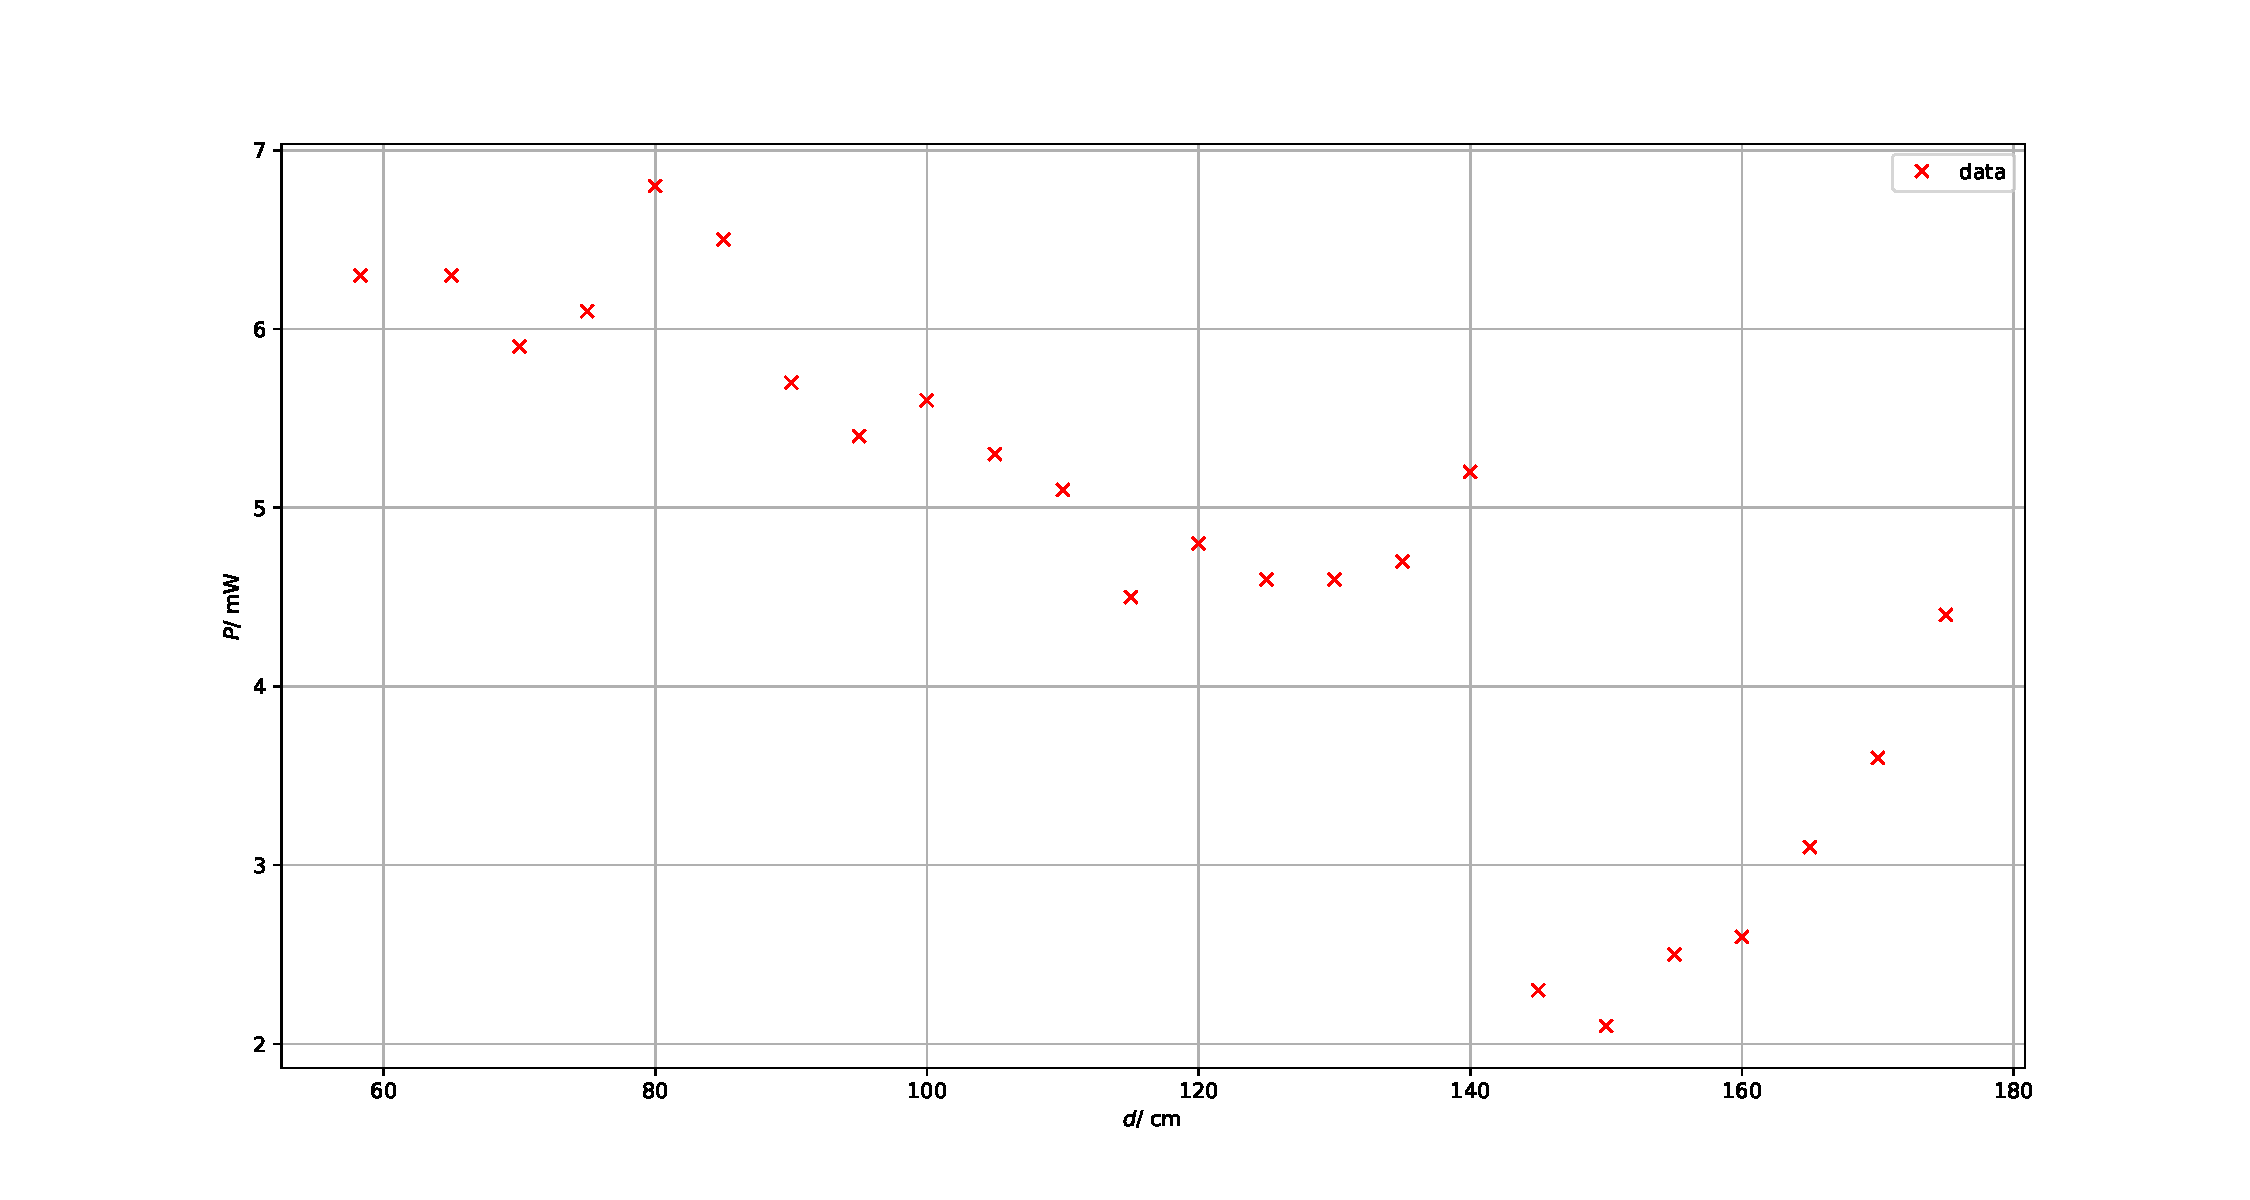
\includegraphics[width=\textwidth]{plots/stability140.pdf}
    \caption{Die Resonatorlänge ist gegen die Leistung aufgetragen. Dabei besteht der Resonator aus zwei konkaven Spiegeln mit jeweils $b_\text{i} = \SI{140}{\centi\meter}$.}
    \label{fig:stability140}
\end{figure} 

Die Stabilität wird auch für einen konkaven Spiegel mit Radius $\SI{140}{\centi\meter}$ in Kombination mit einem flachen Spiegel betrachtet. Die Werte sind in Tab. \ref{tab:stab2} eingetragen. Dargestellt sind diese in Abb. \ref{fig:stability_flat}.
Hier ist bei der Grenze von \SI{140}{\centi\meter} keine Leistung mehr zu messen.

\begin{table}\caption{Die TEM$_{00}$-Mode.}
    \label{tabb}
    \centering
    \sisetup{round-mode = places, round-precision=1, round-integer-to-decimal=true}
    \begin{tabular}{S[] S[]} 
    \toprule
    {$\x / \si{\milli\meter}$} & {$P / \si{\milli\watt}$} \\
    \midrule
    53.0  &  5.5 \\
    60.0  &  2.8 \\
    65.0  &  3.3 \\
    70.0  &  3.1 \\
    75.0  &  3.5 \\
    80.0  &  3.3 \\
    85.0  &  2.8 \\
    90.0  &  3.4 \\
    95.0  &  4.1 \\
    100.0 &  4.6 \\
    105.0 &  5.1 \\
    110.0 &  5.1 \\
    115.0 &  5.1 \\
    120.0 &  4.5 \\
    125.0 &  4.5 \\
    130.0 &  4.3 \\
    135.0 &  3.5 \\
    140.0 &  0.3 \\                  
    \bottomrule
\end{tabular}\end{table}
    

\begin{figure}
    \centering
    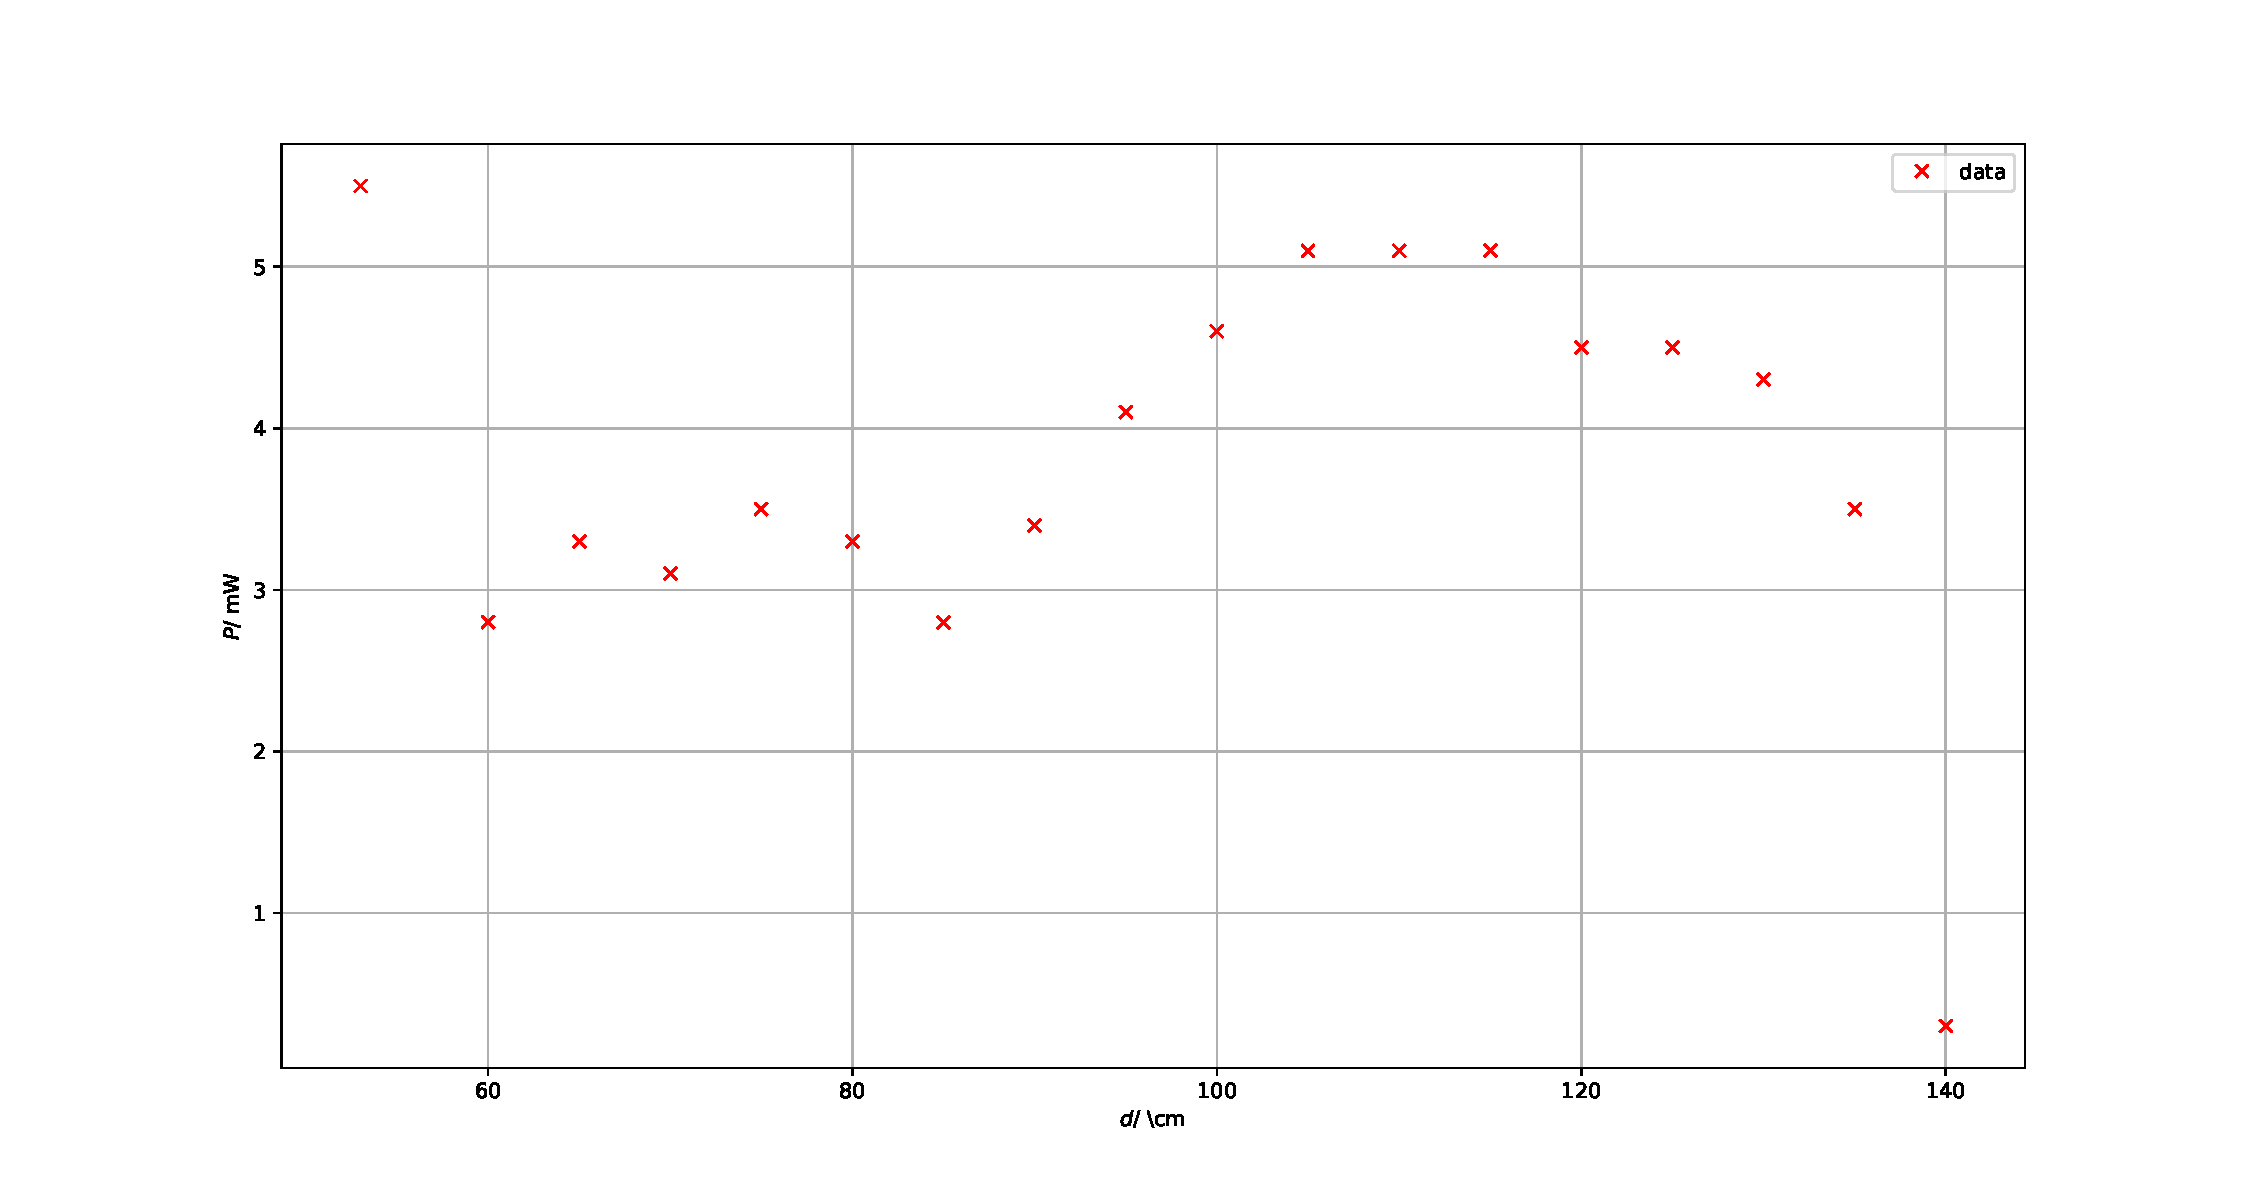
\includegraphics[width=15cm]{plots/stability_flat.pdf}
    \caption{Die Resonatorlänge ist gegen die Leistung aufgetragen. Dabei besteht der Resonator aus einem flachen und einem konkaven Spiegel mit $b_2 = \SI{140}{\centi\meter}$.}
    \label{fig:stability_flat}
\end{figure} 

\subsection{Vermessung von TEM-Moden}

Die gemessenen Werte der TEM$_{00}$-Mode sind in Tab. \ref{tab:mode0} eingetragen und in Abb. \ref{fig:mode0} abgebildet. 
Die Funktionsparameter lassen sich entsprechend dem in Sektion {sec:model} beschriebenen Model mit Formel \eqref{eq:mode0} beschreiben.
\begin{table}\caption{Die TEM$_{00}$-Mode.}
    \label{tabb}
    \centering
    \sisetup{round-mode = places, round-precision=1, round-integer-to-decimal=true}
    \begin{tabular}{S[] S[] S[] S[]} 
    \toprule
    {$x / \si{\milli\meter}$} & {$I / \si{\micro\ampere}$} & {$x / \si{\milli\meter}$} & {$I / \si{\micro\ampere}$} \\
    \midrule
    0.0    &    0.3  &   10.5   &    3.4      \\     
    0.5    &    0.7  &   11.0   &    1.6      \\     
    1.0    &    1.7  &   11.5   &    0.8      \\     
    1.5    &    3.8  &   12.0   &    0.5      \\     
    2.0    &    7.9  &   12.5   &    0.3      \\ 
    2.5    &    15.8 &          &             \\ 
    3.0    &    27.8 &          &             \\ 
    3.5    &    41.4 &          &             \\ 
    4.0    &    58.0 &          &             \\ 
    4.5    &    75.3 &          &             \\ 
    5.0    &    88.3 &          &             \\ 
    5.5    &    94.8 &          &             \\ 
    6.0    &    93.5 &          &             \\ 
    6.5    &    84.2 &          &             \\ 
    7.0    &    71.7 &          &             \\ 
    7.5    &    60.4 &          &             \\ 
    8.0    &    48.1 &          &             \\ 
    8.5    &    36.1 &          &             \\ 
    9.0    &    23.5 &          &             \\ 
    9.5    &    13.6 &          &             \\ 
    10.0   &    7.4  &          &             \\        
    \bottomrule
\end{tabular}\end{table}
    

\begin{figure}
    \centering
    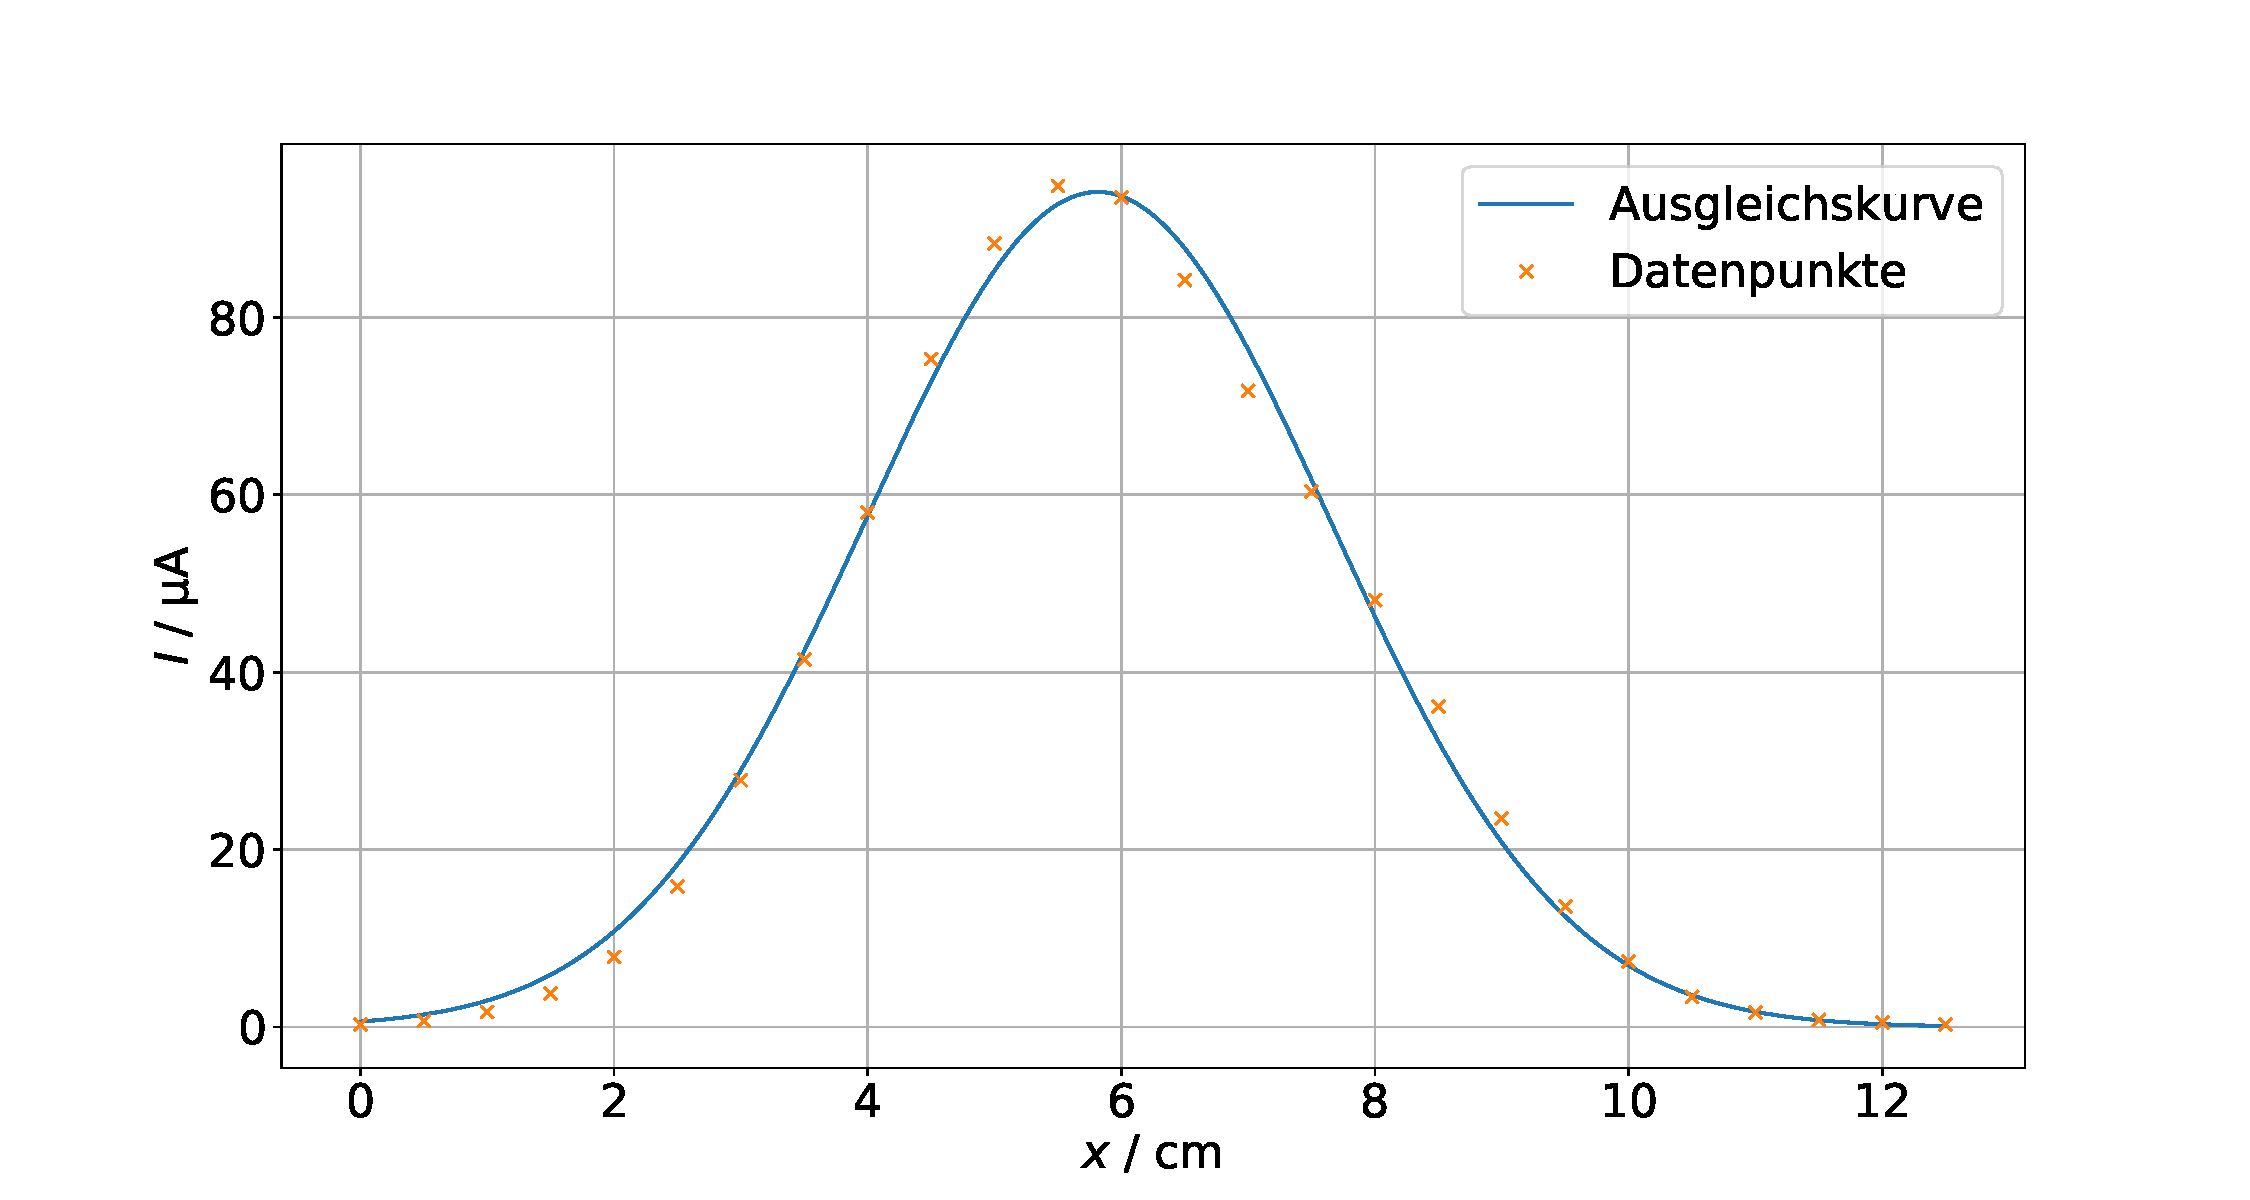
\includegraphics[width=\textwidth]{plots/mode0.pdf}
    \caption{Der Abstand senkrecht zur Laserachse ist gegen die gemessene Stromstärke aufgetragen. Zu sehen ist die TEM$_{00}$-Mode.}
    \label{fig:mode0}
\end{figure}

Die Fitparameter ergeben sich zu 
\begin{align*}
    \mu &= \SI{5.814(23)}{\centi\meter} \\
    w &= \SI{2.592(33)}{\centi\meter} \\ 
    I_0 &= \SI{316(7)}{\micro\ampere}.
\end{align*}


Die gemessenen Werte der TEM$_{10}$-Mode sind in Tab. \ref{tab:mode1} eingetragen und in Abb. \ref{fig:mode1} abgebildet. 
Die Funktionsparameter lassen sich mit Formel \eqref{eq:mode1} modellieren.

\begin{table}\caption{Die TEM$_{10}$-Mode. Der Abstand senkrecht zur Laserachse ist gegen die Stromstärke aufgelistet.}
    \label{tab:mode1}
    \centering
    \sisetup{round-mode = places, round-precision=1, round-integer-to-decimal=true}
    \begin{tabular}{S[] S[] | S[] S[] | S[] S[] | S[] S[] | S[] S[]} 
    \toprule
    {$x / \si{\milli\meter}$} & {$I / \si{\micro\ampere}$} & {$x / \si{\milli\meter}$} & {$I / \si{\micro\ampere}$} & {$x / \si{\milli\meter}$} & {$I / \si{\micro\ampere}$} & {$x / \si{\milli\meter}$} & {$I / \si{\micro\ampere}$} & {$x / \si{\milli\meter}$} & {$I / \si{\micro\ampere}$} \\
    \midrule
0.00    &    0.1  & 2.75    &    5.4  &  5.50    &    4.1   &   8.25    &    7.8    & 11.00   &    4.2   \\
0.25    &    0.14 & 3.00    &    6.4  &  5.75    &    2.6   &   8.50    &    8.6    & 11.25   &    3.3   \\
0.50    &    0.23 & 3.25    &    7.3  &  6.00    &    1.1   &   8.75    &    9.1    & 11.50   &    2.4   \\
0.75    &    0.40 & 3.50    &    8.1  &  6.25    &    0.4   &   9.00    &    10.3   & 11.75   &    1.4   \\
1.00    &    0.68 & 3.75    &    9.7  &  6.50    &    0.3   &   9.25    &    9.7    & 12.00   &    0.9   \\
1.25    &    1.09 & 4.00    &    10.6 &  6.75    &    0.7   &   9.50    &    8.9    & 12.25   &    0.7   \\
1.50    &    1.6  & 4.25    &    11.6 &  7.00    &    1.4   &   9.75    &    8.4    & 12.50   &    0.4   \\
1.75    &    2.3  & 4.50    &    10.7 &  7.25    &    2.4   &   10.00   &    7.9    & 12.75   &    0.3   \\
2.00    &    3.0  & 4.75    &    9.7  &  7.50    &    3.6   &   10.25   &    7.1    &         &          \\
2.25    &    3.6  & 5.00    &    8.4  &  7.75    &    4.9   &   10.50   &    6.7    &         &          \\
2.50    &    4.5  & 5.25    &    6.7  &  8.00    &    6.5   &   10.75   &    5.1    &         &          \\ 

    \bottomrule
\end{tabular}\end{table}
    

\begin{figure}
    \centering
    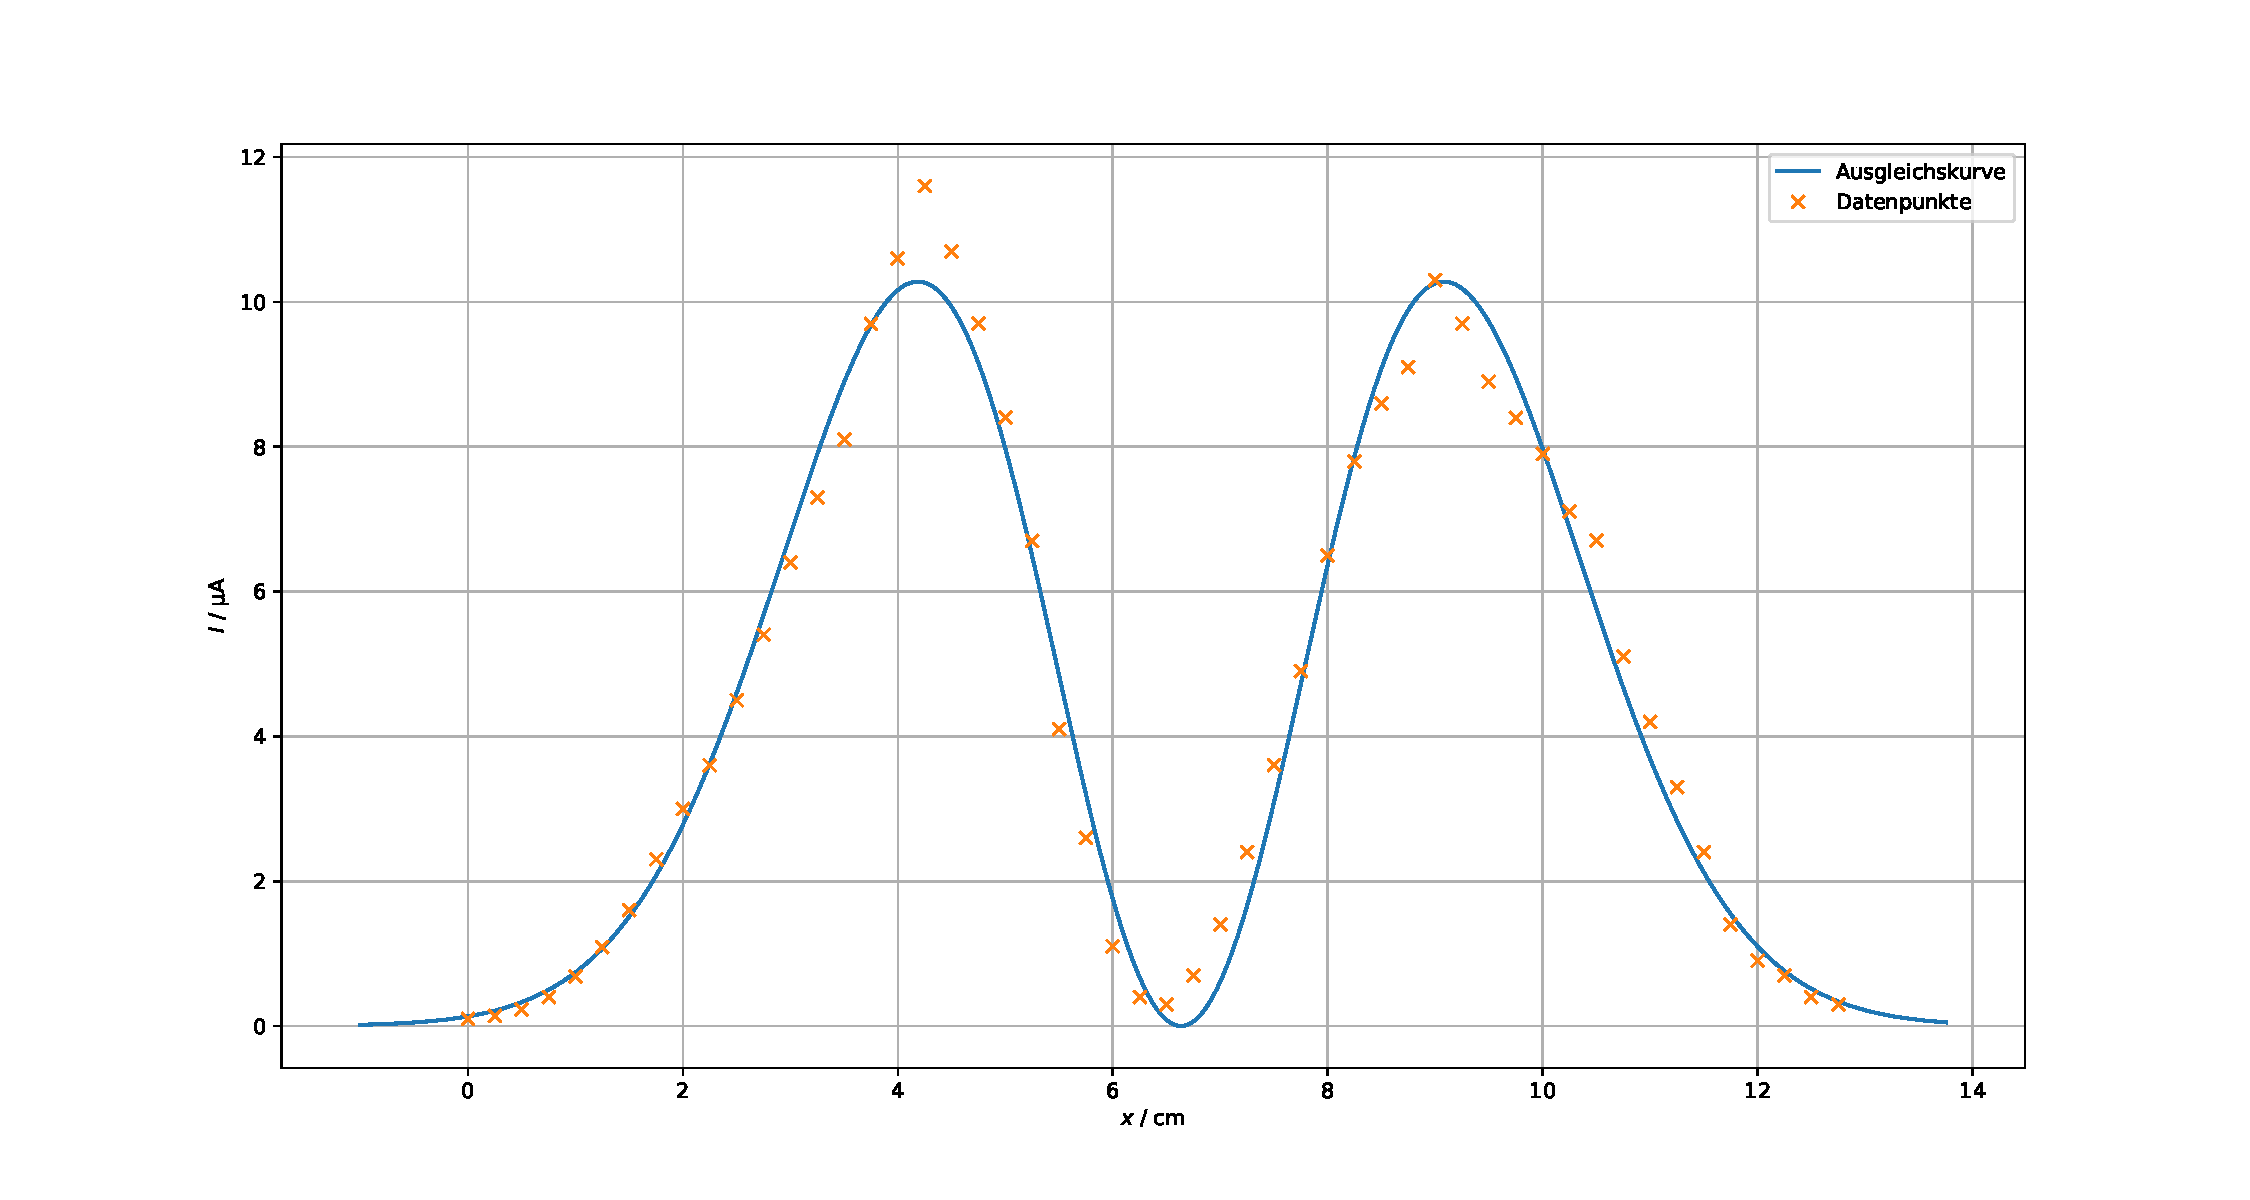
\includegraphics[width=15cm]{plots/mode1.pdf}
    \caption{Der Abstand senkrecht zur Laserachse ist gegen die gemessene Stromstärke aufgetragen. Zu sehen ist die TEM$_{10}-$Mode.}
    \label{fig:mode1}
\end{figure}

Die Fitparameter ergeben sich zu 
\begin{align*}
    \mu &= \SI{6.634(18)}{\centi\meter} \\
    w &= \SI{2.447(18)}{\centi\meter} \\ 
    I_0 &= \SI{10.46(17)}{\micro\ampere}.
\end{align*}

Die gemessenen Werte der TEM$_{20}$-Mode sind in Tab. \ref{tab:mode2} eingetragen und in Abb. \ref{fig:mode2} abgebildet. 
Die Funktionsparameter lassen sich mit Formel \eqref{eq:mode2} modellieren.

\begin{table}\caption{Die TEM$_{20}$-Mode.}
    \label{tabb}
    \centering
    \sisetup{round-mode = places, round-precision=2, round-integer-to-decimal=true}
    \begin{tabular}{S[] S[] S[] S[] S[] S[]} 
    \toprule
    {$x / \si{\milli\meter}$} & {$I / \si{\micro\ampere}$} & {$x / \si{\milli\meter}$} & {$I / \si{\micro\ampere}$} & {$x / \si{\milli\meter}$} & {$I / \si{\micro\ampere}$}\\
    \midrule
0.00    &    0.24 & 5.25    &    0.08 & 10.50   &    0.70     \\
0.25    &    0.35 & 5.50    &    0.13 & 10.75   &    0.65     \\
0.50    &    0.46 & 5.75    &    0.22 & 11.00   &    0.51     \\
0.75    &    0.60 & 6.00    &    0.30 & 11.25   &    0.44     \\
1.00    &    0.65 & 6.25    &    0.36 & 11.50   &    0.32     \\
1.25    &    0.9  & 6.50    &    0.43 & 11.75   &    0.26     \\
1.50    &    0.95 & 6.75    &    0.34 & 12.00   &    0.18     \\
1.75    &    1.1  & 7.00    &    0.32 & 12.25   &    0.14     \\
2.00    &    1.0  & 7.25    &    0.34 & 12.50   &    0.1      \\
2.25    &    0.97 & 7.50    &    0.24 & 12.75   &    0.06     \\
2.50    &    0.98 & 7.75    &    0.16 & 13.00   &    0.04     \\
2.75    &    0.84 & 8.00    &    0.06 &         &             \\
3.00    &    0.75 & 8.25    &    0.05 &         &             \\
3.25    &    0.57 & 8.50    &    0.11 &         &             \\
3.50    &    0.43 & 8.75    &    0.21 &         &             \\
3.75    &    0.35 & 9.00    &    0.27 &         &             \\
4.00    &    0.22 & 9.25    &    0.43 &         &             \\
4.25    &    0.11 & 9.50    &    0.65 &         &             \\
4.50    &    0.06 & 9.75    &    0.72 &         &             \\
4.75    &    0.03 & 10.00   &    0.76 &         &             \\
5.00    &    0.04 & 10.25   &    0.80 &         &             \\






















    \bottomrule
    \end{tabular}
\end{table}
    

\begin{figure}
    \centering
    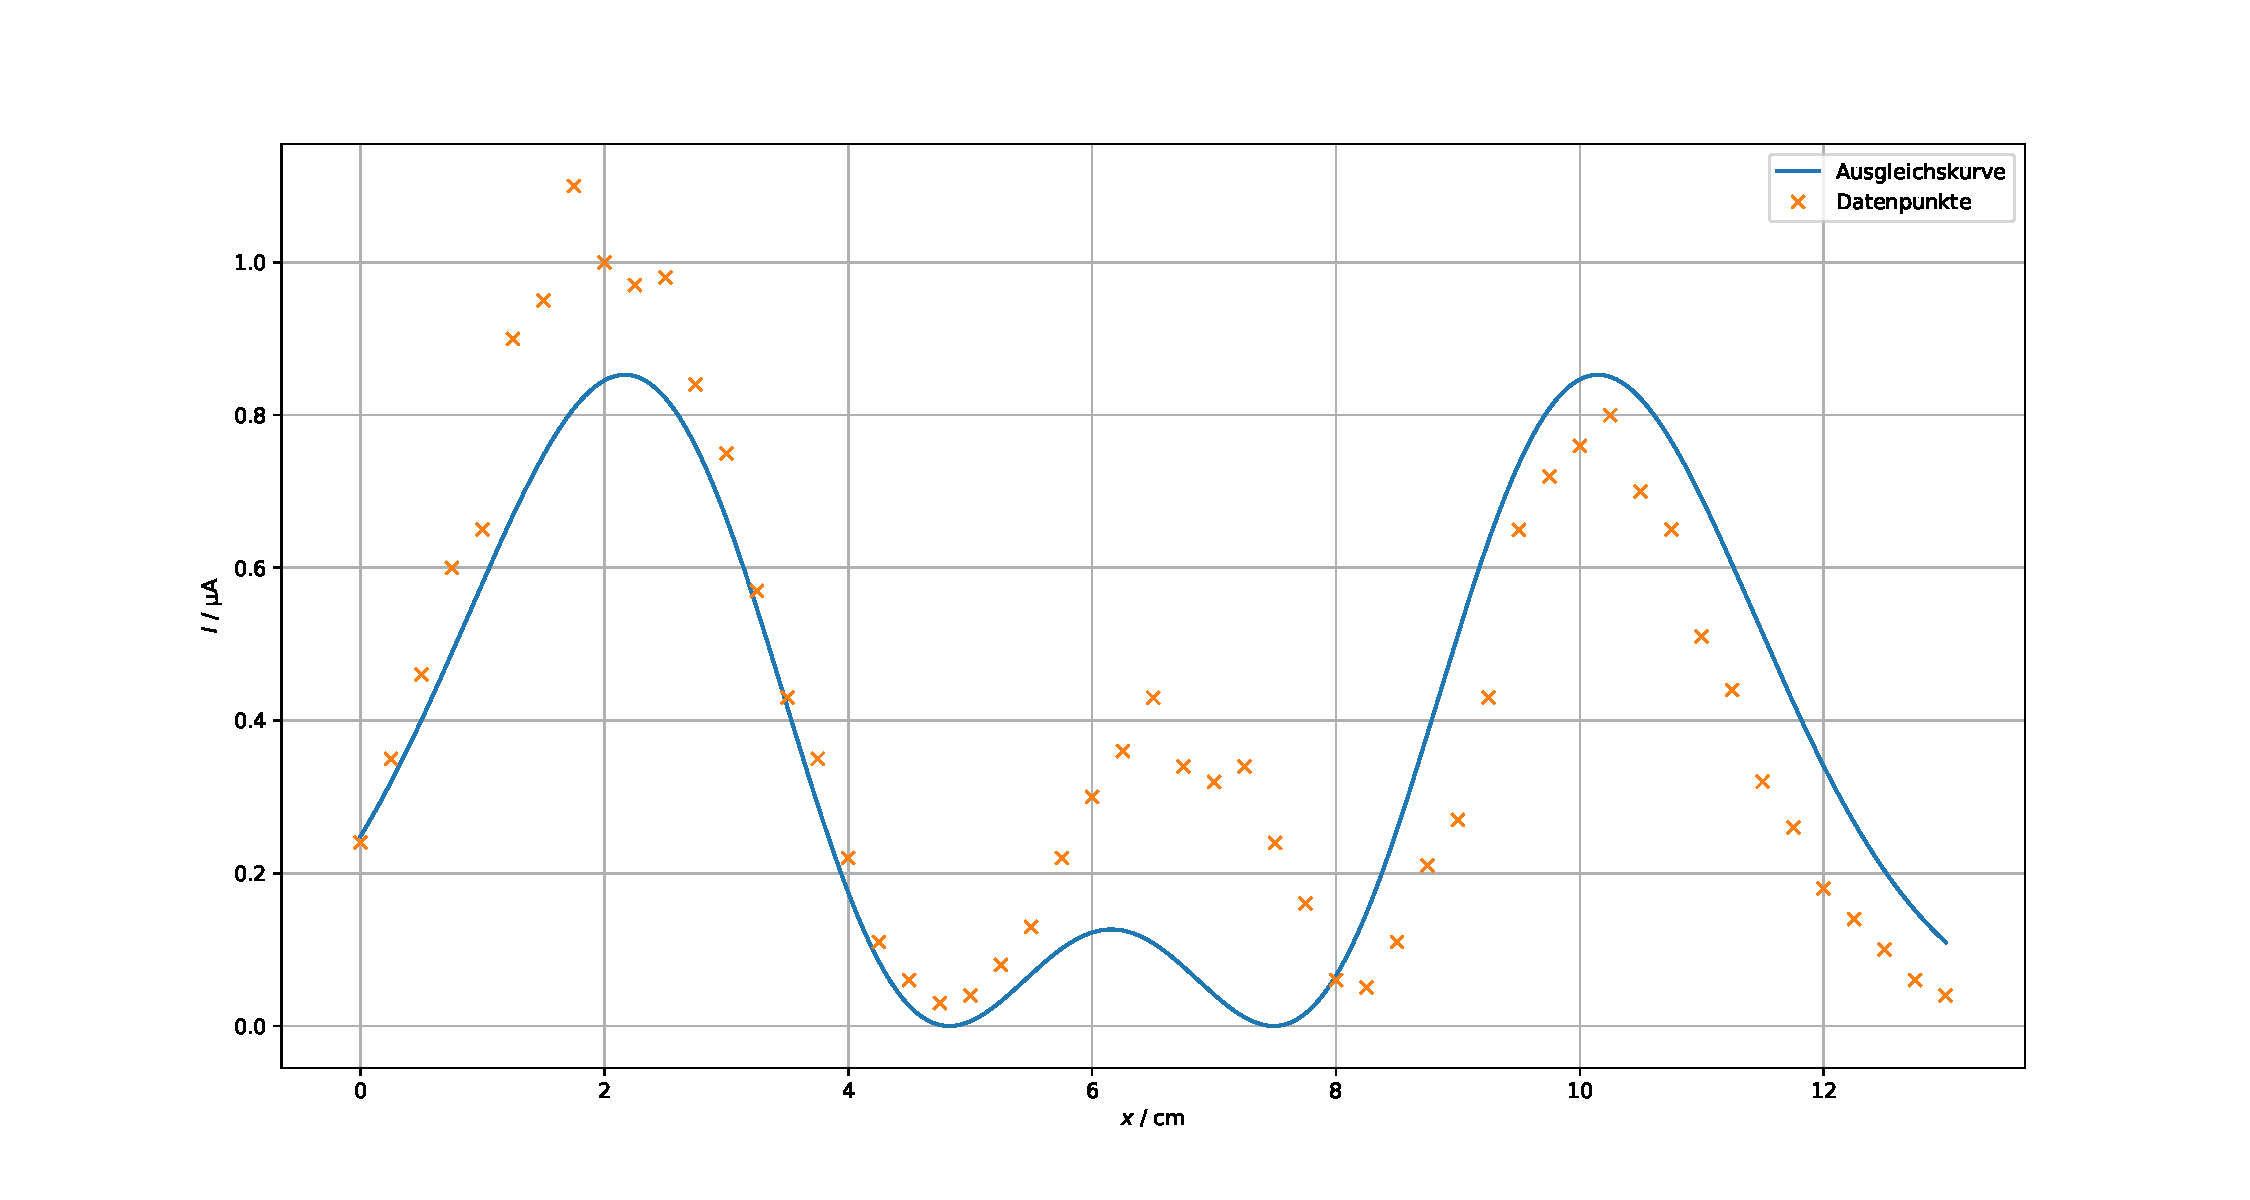
\includegraphics[width=15cm]{plots/mode2.pdf}
    \caption{Der Abstand senkrecht zur Laserachse ist gegen die gemessene Stromstärke aufgetragen. Zu sehen ist die TEM$_{20}-$Mode.}
    \label{fig:mode2}
\end{figure}

Die Fitparameter ergeben sich zu 
\begin{align*}
    \mu &= \SI{6.16(7)}{\centi\meter} \\
    w &= \SI{2.66(5)}{\centi\meter} \\ 
    I_0 &= \SI{0.112(6)}{\micro\ampere}.
\end{align*}

\subsection{Messung der Polarisation}

Die bestimmten Werte der Polarisation ergeben sich aus Tab. \ref{tab:polar} und sind in Abb. \ref{fig:polarisation} dargestellt. 
\begin{table}\caption{Die Werte zur Beschreibung der Polarisation. Es sind die Winkel und die Leistung gegeneinander aufgelistet.}
    \label{tab:polar}
    \centering
    \sisetup{round-mode = places, round-precision=1, round-integer-to-decimal=true}
    \begin{tabular}{S[] S[] | S[] S[]} 
    \toprule
    {$\phi / \si{\degree}$} & {$P / \si{\milli\watt}$} & {$\phi / \si{\degree}$} & {$P / \si{\milli\watt}$}  \\
    \midrule
    0   & 0.86 &  180 & 0.9    \\
    20  & 0.1  & 200 & 0.11  \\
    40  & 0.33 & 220 & 0.28  \\
    60  & 1.51 & 240 & 1.31  \\
    80  & 2.88 & 260 & 2.82  \\ 
    100 & 3.91 & 280 & 4.05  \\
    120 & 4.40 & 300 & 4.43  \\ 
    140 & 3.66 & 320 & 3.71  \\ 
    160 & 2.3  & 340 & 2.36  \\                                    
    \bottomrule
\end{tabular}\end{table}
    

\begin{figure}
    \centering
    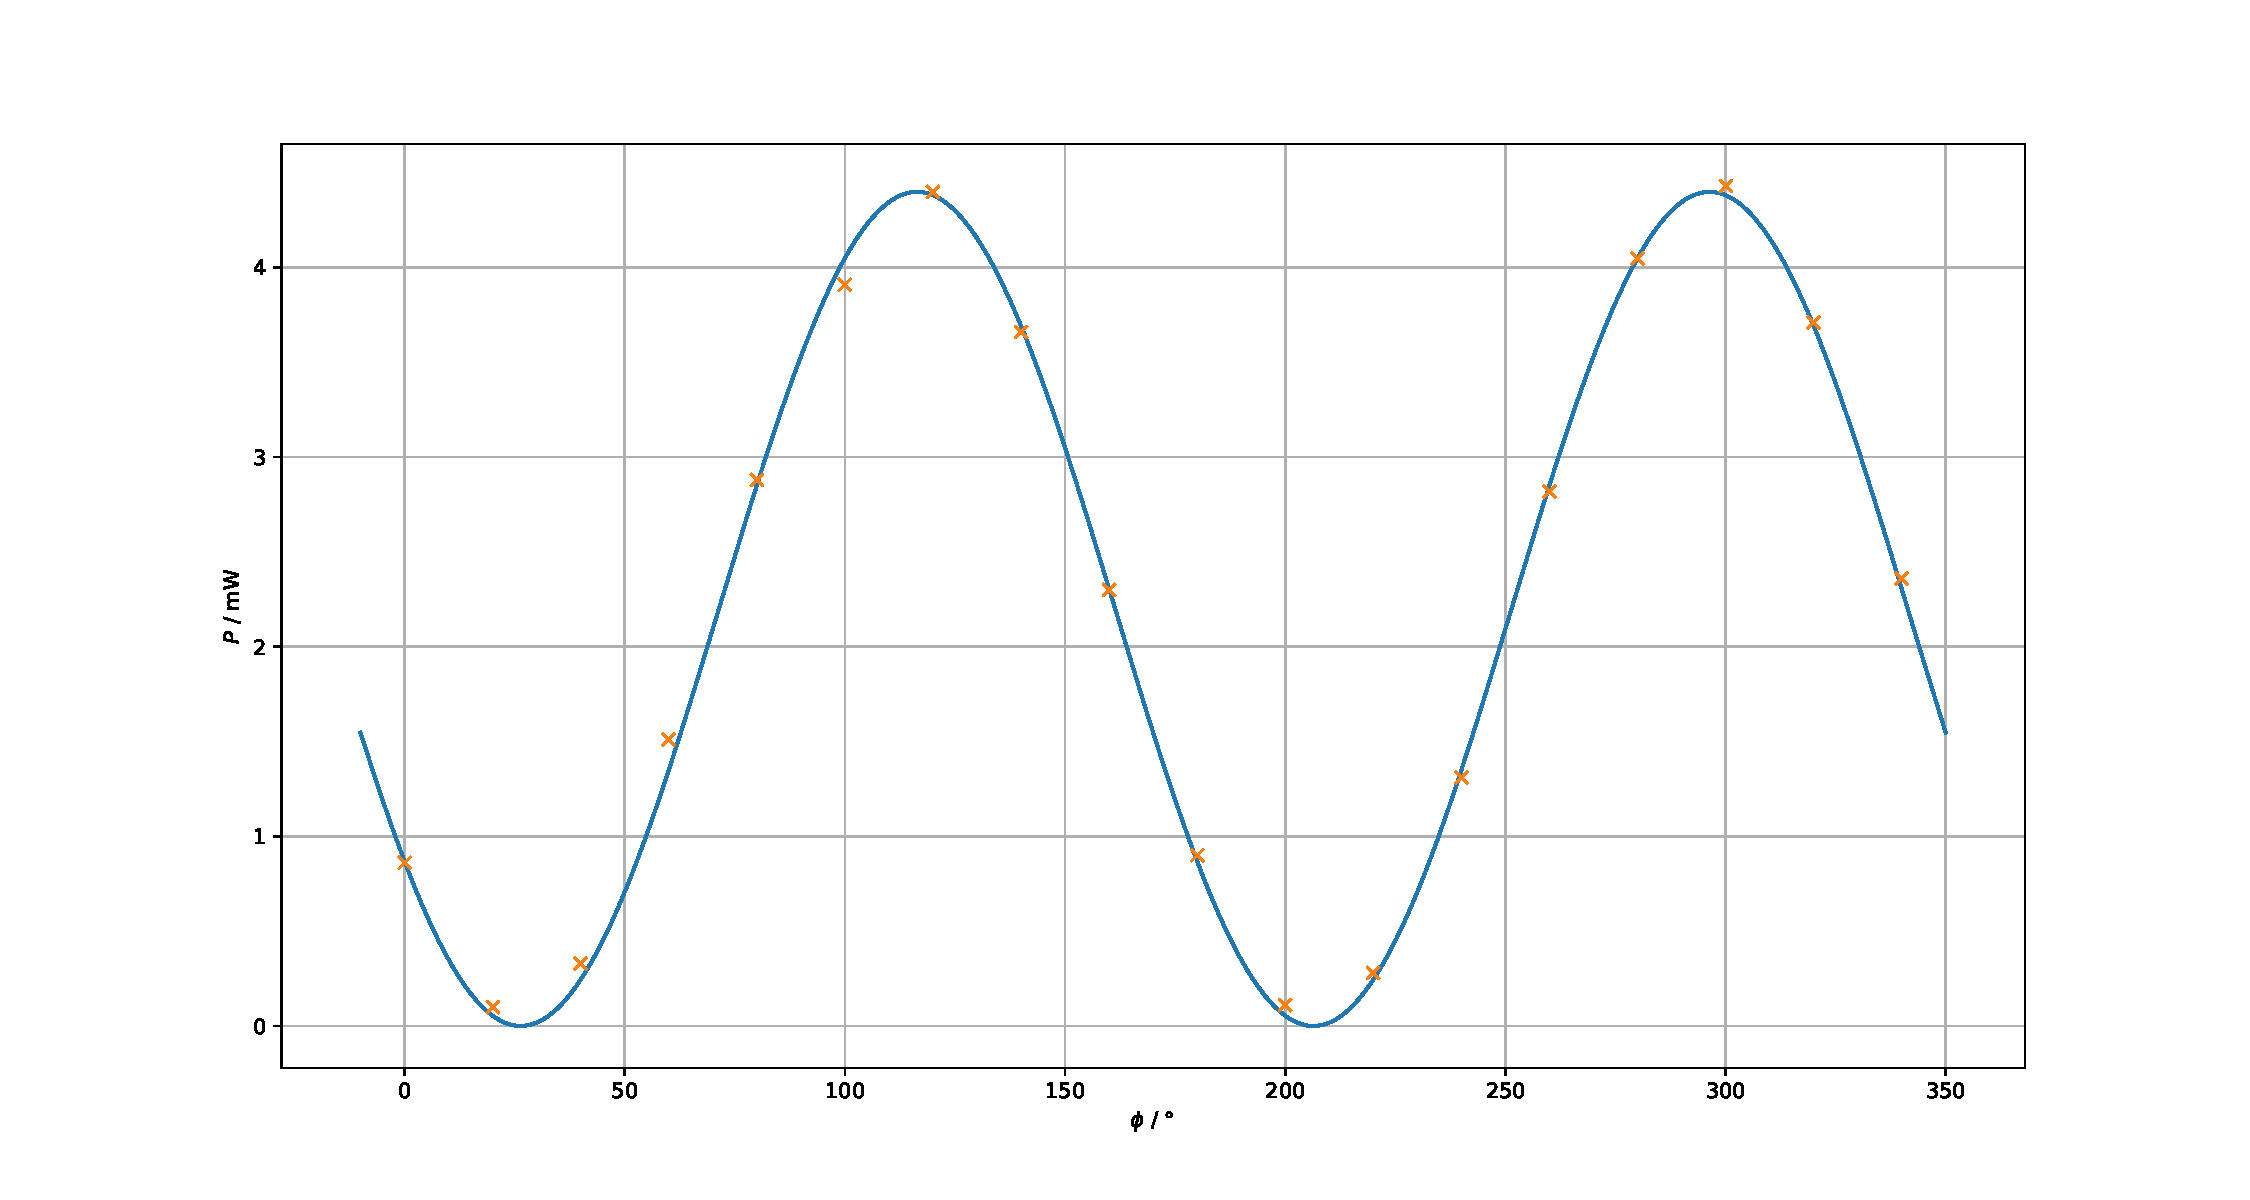
\includegraphics[width=15cm]{plots/polarisation.pdf}
    \caption{Der Polarisationswinkel ist gegen die Leistung aufgetragen.}
    \label{fig:polarisation}
\end{figure}    

Die Messung ist mit dem in Formel \eqref{eq:polar} beschriebenen Model gefittet. Die Fitparameter ergeben sich zu 
\begin{align*}
    P_0 &= \SI{4.399(26)}{\milli\watt} \\
    \delta &= \SI{63.63(29)}{\degree}.
\end{align*}

\subsection{Bestimmung der Wellenlänge}

Die Wellenlänge des Lasers wird mit verschiedenen Gittern bestimmt. 
Dazu wird sowohl der Abstand zwischen drei verschiedenen Gittern und Schirm, als auch jeweils der Abstand der Maxima auf dem Schirm bestimmt. 

Mit Formel \eqref{eq:welle} kann somit jeweils die Wellenlänge berechnet werden. 
Die gemessenen Daten und berechneten Ergebnisse für drei verschiedene Gitter sind in Tab. \ref{tab:welle} eingetragen. 

\begin{table}\caption{Die Daten und Ergebnisse der Wellenlängen-Messung.}
    \label{tab:welle}
    \centering
    \sisetup{round-mode = places, round-integer-to-decimal=true}
    \begin{tabular}{c S[] S[] S[]} 
    \toprule
    {Gitter} & {$d / \si{\centi\meter}$} & {$a / \si{\centi\meter}$} & {$\lambda / \si{\nano\meter}$} \\
    \midrule

    \phantom{1}80/\si{\milli\meter} & 22.5 & 1.2 & 665.72 \\
    100/\si{\milli\meter}           & 32.5 & 2.1 & 644.81 \\
    600/\si{\milli\meter}           & 12.5 & 5.3 & 650.60 \\


    \bottomrule
\end{tabular}\end{table}
    